\documentclass[10pt,landscape]{article}
\usepackage{multicol}
\usepackage{calc}
\usepackage{ifthen}
\usepackage[landscape]{geometry}
\usepackage{amsmath,amsthm,amsfonts,amssymb}
\usepackage{color,graphicx,overpic}
\usepackage{tikz}
\usepackage{tikz-3dplot}


\pdfinfo{
  /Title (physics.pdf)
  /Creator (TeX)
  /Producer (pdfTeX 1.40.0)
  /Author (Kevin)
  /Subject (Physics Cheat Sheet)
  /Keywords (physics, tex, latex)}

\geometry{top=.5in,left=.5in,right=.5in,bottom=.5in}

% Turn off header and footer
\pagestyle{empty}

% Redefine section commands to use less space
\makeatletter
\renewcommand{\section}{\@startsection{section}{1}{0mm}%
                                {-1ex plus -.5ex minus -.2ex}%
                                {0.5ex plus .2ex}%
                                {\normalfont\large\bfseries}}
\renewcommand{\subsection}{\@startsection{subsection}{2}{0mm}%
                                {-1explus -.5ex minus -.2ex}%
                                {0.5ex plus .2ex}%
                                {\normalfont\normalsize\textit}}
\renewcommand{\subsubsection}{\@startsection{subsubsection}{3}{0mm}%
                                {-1ex plus -.5ex minus -.2ex}%
                                {1ex plus .2ex}%
                                {\normalfont\small\underline}}
\makeatother

\renewcommand{\baselinestretch}{1.5}

% Don't print section numbers
\setcounter{secnumdepth}{0}


\setlength{\parindent}{0pt}
\setlength{\parskip}{0pt plus 0.5ex}

%My Environments
\newtheorem{example}[section]{Example}
% -----------------------------------------------------------------------

\begin{document}
\raggedright
\footnotesize
\begin{multicols}{3}


% multicol parameters
% These lengths are set only within the two main columns
%\setlength{\columnseprule}{0.25pt}
\setlength{\premulticols}{1pt}
\setlength{\postmulticols}{1pt}
\setlength{\multicolsep}{1pt}
\setlength{\columnsep}{2pt}

\begin{center}
     \Large{\textbf{Physics}} \\
\end{center}

\section{Kinematics}
$\overline{v}=\frac{\Delta{x}}{\Delta{t}}$ (SI: $\frac{\text{m}}{\text{s}}$)\newline
$a=\frac{\Delta v}{\Delta t}$ (SI: $\frac{\text{m}}{\text{s\textsuperscript{2}}}$)

\subsection{Linear Motion}
$v=v_{0}+at$ \newline
$x=v_{0}t+\frac{1}{2}at^{2}$ \newline
$v^{2}=v_{0}^{2}+2ax $ \newline
$\overline{v}=\frac{(v_{0}+v)}{2}$ \newline
$x=\overline{v}t$

\subsection{Slopes}
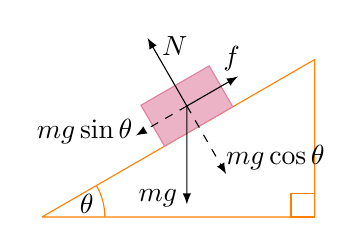
\begin{tikzpicture}

\newcommand{\ang}{30}
\draw [draw = orange, fill = orange!0] (0,0) coordinate (O) -- (\ang:4)
    coordinate [pos=.45] (M) |- coordinate (B) (O);

\draw [draw = orange] (O) ++(.8,0) arc (0:\ang:0.8) 
    node [pos=.4, left] {$\theta$};
\draw [draw = orange] (B) rectangle ++(-0.3,0.3);

\begin{scope} [-latex,rotate=\ang]
 
% Object (rectangle)
\draw [fill = purple!30,
    draw = purple!50] (M) rectangle ++ (1,.6);
 
% Weight Force and its projections
\draw [dashed] (M) ++ (.5,.3) coordinate (MM) -- ++ (0,-1)
    node [near end, right] {$mg\cos{\theta}$};
 
\draw [dashed] (MM) -- ++ (-0.75,0) 
    node [very near end, left] {$mg\sin{\theta}$};
 
\draw (MM) -- ++ (-\ang-90:1.25)
    node [near end,below left ] {$mg$};
 
% Normal Force
\draw (MM) -- ++ (0,1)
node [very near end, right] {$N$};
 
% Frictional Force
\draw (MM) -- ++ (0.75,0)
    node [very near end, above] {$f$};
 
\end{scope}

\end{tikzpicture}


\section{Newton's Laws}
$F=ma$ (SI: N)

\subsection{Gravity}
$F=\frac{Gm_{1}m_{2}}{r^{2}}$ \newline
$g=G\frac{M}{r^{2}}$

\subsection{Circular Motion}
$a_{c}=\frac{v^{2}}{r}$ (SI: $\frac{\text{m}}{\text{s}^{2}}$) \newline
$F_{c}=\frac{mv^{2}}{r}$ (SI: N)

\subsection{Torque}
Center of Mass: $x \textsubscript{cm}= \frac{\sum m_{i}x_{i}}{M}$ \newline
Torque: $\tau =rF \sin{\theta} $ (SI: N$\cdot$m)

\subsection{Mechanical Advantage}
$F_{1} \cdot d_{1}= F_{2} \cdot d_{2}$ \newline
Mechanical Advantage: $\text{MA}=\frac{F_\text{in}}{F_{\text{out}}}$

\section{Work Energy Power}
Work: $W=Fd$ (SI: J) \newline
P: $P= \frac{W}{\Delta t}$ (SI: W) \newline
KE: $K=\frac{1}{2}mv^{2}$ \newline
PE: $U=mgh$\newline
$W=\Delta{K}=- \Delta{U}$ \newline
$E=K+U$

\subsection{Springs}
Hooke's Law: $F=-kx$ \newline
Potential Energy: $U=\frac{1}{2}kx^{2}$

\section{Thermodynamics}

\subsection{Thermal Expansion}
Linear: \space $\Delta L = \alpha L\Delta T$ \newline
Volume: $\Delta V = \beta V\Delta T$ 

\subsection{Specific Heat}
$Q=mc\Delta T$ \newline	
$U= Q - W$ \newline
Water s.h.c. : 1 cal g\textsuperscript{-1} K\textsuperscript{-1} =  4.2 J g\textsuperscript{-1} K\textsuperscript{-1}

\section{Fluid Dynamics}
$\rho=\frac{m}{V}$ (SI: $\frac{\text{kg}}{\text{m\textsuperscript{3}}}$)\newline
Weight = $\rho gV$ (SI: N) \newline
Specific Gravity = $\frac{\rho _{\text{substance}}}{\rho _{\text{water}}} ; \ \rho_{\text{water}}=1000$ kg m\textsuperscript{-3})

\subsection{Pressure}
$P=\frac{F}{A}$ (SI: Pa) \newline
Hydrostatic: $P_{h}=\rho gh$ \newline
Gauge: $P_{g}=P-P_{atm}$ \newline
Absolute: $\sum P$ \newline
1 atm = 760 torr = 760 mmHg = 10\textsuperscript{5} Pa 

\subsection{Flow}
Continuity Equation: $A_{1}v_{1}=A_{2}v_{2}$ \newline
Bernoulli's Equation: $P+\frac{1}{2}\rho v^{2}+\rho g h =$ constant \newline
Poiseuille: $Q=\frac{\pi P r^{4}}{8 \eta l}; \ \eta \rightarrow$viscosity \newline
Reynold's Numnber: $v_{\text{critical}}= \frac{R \eta}{2 \rho r}$

\subsection{Principles}
Archimedes: $F_{\text{buoy}}=g\cdot \rho_{\text{fluid}}\cdot V_{\text{submerged}}$ \newline
Pascal:\newline
\-\hspace{0.5 cm}$P=\frac{F_{1}}{A_{1}}=\frac{F_{2}}{A_{2}}$ \newline
\-\hspace{0.5 cm}$A_{1}d{1}=A_{2}d_{2}$ \newline
\-\hspace{0.5 cm}$W=F_{1}{d_{1}=F_{2}}d_{2}$ 


\section{Electrostatics}
Coulomb's Law: $F=\frac{kq_{1}q_{2}}{r^{2}}; k=9\cdot 10^{9}$ N $\cdot$ m\textsuperscript{2} $\cdot$ C\textsuperscript{-2} (SI:N)

\subsection{Electric Fields}
Electric Field Equation: $E=\frac{F_{\text{e}}}{q}=\frac{kQ}{r^{2}}$ (SI:$\frac{\text{N}}{\text{C}}$ or $\frac{\text{V}}{\text{M}}$) \newline 
\fbox{\begin{minipage}{25 em}
Electric field lines go from $+$ to $-$ \newline
$+$ charge moves in the same direction of the electric field \newline
$-$ charge moves in the opposite direction
\end{minipage}}
\newline

\subsection{Electric Dipoles}
Dipole Moment: $p=q\cdot d$ (SI: C$\cdot $m)\newline
$F_{\text{e}}=qE$ \newline
$\sum F_{e}=0$ \newline
\fbox{Dipole will realign to be parallel with an electric field}

\subsection{Electrical Potential}
Voltage: $V=\frac{U}{q}$ (SI: V or $\frac{\text{J}}{\text{C}}$) \newline
Voltage Difference: $\Delta V=\frac{W}{q}=\frac{kQ}{r}=Ed$ (SI: V or $\frac{\text{J}}{\text{C}}$) \newline
\fbox{\begin{minipage}{25 em}
Voltage is the amount of work to move a postitive test charge from infinity to some location
\end{minipage}} \newline

\section{Magnetism}
$F_{\text{m}}=Q \cdot v \cdot  \beta \cdot \sin{\theta};$  (SI: $\beta \rightarrow$T)\newline
Lorentz Force: $F=F_{\text{m}}+ F_{\text{e}}$

\subsection{Right Hand Rule}
\tikzset{
    axis/.style={-stealth,line width=2pt,every node/.append style={text=black}},
    xaxis/.style={axis,red},
    yaxis/.style={axis,green},
    zaxis/.style={axis,blue},
}

\tdplotsetmaincoords{60}{230}
\begin{tikzpicture}[tdplot_main_coords]
	\draw[xaxis] (0,0,0) -- (1,0,0) node[pos=1.5]{\text{Current}};
   	\draw[yaxis] (0,0,0) -- (0,1,0) node[pos=1.7]{\text{Magnetic Field}};
	\draw[zaxis] (0,0,0) -- (0,0,1) node[pos=1.3]{\text{Force}};
	\shade [ball color=black] (0,0,0) circle [radius=0.06cm];
\end{tikzpicture}

\subsection{Electromagnetism}
$F_{\text{m}}= I \cdot L \cdot \beta \cdot sin{\theta}$ \newline
Biot-Savart Law: $\beta=\frac{\mu_{0}I}{2 \pi R}$


\section{Circuits}
Current: $I=\frac{Q}{\Delta t}$ (SI: A) \newline
Resistance: $ R = \frac{\rho L}{A}; \ \rho \rightarrow \text{resistivity, A}\rightarrow \text{area}$ (SI: $\Omega $)
Voltage: $V=IR$ (SI: V) \newline
Power: $P=IV$ (SI: W)\newline
Capacitance: $C=\frac{Q}{V}$ (SI: F) 

\subsection{Resistors}
Series: $R_{eq}=R_{1}+R_{2}+R_{3}+ ...$ \newline
Parallel: $\frac{1}{R_{\text{eq}}}=\frac{1}{R_{1}}+\frac{1}{R_{2}}+\frac{1}{R_{3}}+ ...$

\subsection{Capacitors}
Series: $\frac{1}{C_{\text{eq}}}=\frac{1}{C_{1}}+\frac{1}{C_{2}}+\frac{1}{C_{3}}+ ...$ \newline
Parallel: $C_{eq}=C_{1}+C_{2}+C_{3}+ ...$ \newline
Energy Stored: $U=\frac{1}{2}QV=\frac{1}{2}CV^{2}=\frac{1}{2}\frac{Q^{2}}{C}$ \newline
Dielectric: $C_{\text{dielectric}}=kC; k\rightarrow$ dielectric constant



\section{Waves}
$f=\frac{1}{T}$ (SI: Hz) \newline
$v=f \cdot \lambda$ (SI: $\frac{\text{m}}{\text{s}}$)

\subsection{Standing Waves}
Open Pipe: $\lambda=\frac{2L}{n}; \ n\rightarrow 1,2,3 \ldots$ \newline
Closed Pipe: $\lambda\frac{4L}{n}; \ n\rightarrow 1,3,5 \ldots$

\subsection{Sound}
Intensity: $I=\frac{P}{A}$ \newline
Sound Level: $\beta=10 \log(\frac{I}{I_{0}}); \ I_{0}=10^{-12}$ (SI: dB) \newline
Doppler Effect: $f'=f\frac{v \pm v_{\text{d}}}{v \mp v_{\text{s}}}; \ v=343 \frac{\text{m}}{\text{s}}$


\section{Optics}

\subsection{Reflection and Refraction}
$\theta _{\text{incidence}} = \theta _{\text{reflection}}$ \newline
Snell's Law: $n_\text{i} \sin \theta _{\text{i}} = n_r \sin \theta _{\text{r}}$ \newline
Index of Refraction: $n=\frac{c}{v}; \ c=3 \cdot 10^{8} \frac{\text{m}}{\text{s}}$

\subsection{Diffraction}

\subsection{Mirrors and Lenses}
Focal Point: $f=\frac{1}{2}$ radius of curvature \newline
Thin Lens Equation: $\frac{1}{f}=\frac{1}{d_{\text{o}}}+\frac{1}{d_{\text{i}}}$ \newline
Magnification Equation: $M=-\frac{d_{\text{i}}}{d_{\text{o}}}=\frac{h_{\text{i}}}{h_{\text{o}}}$



\end{multicols}
\end{document}